\section{RISULTATI}
Per quanto concerne le analisi relative alle performance (in termini di f1-\textit{score} per i motivi precedenetemente discussi) di DT e RF al variare del numero di feature estratte dal processo di PCA, i risultati (riportati in Figura \ref{fig:pca-perf}) mostrano come per dimensioni basse le performance tra i modelli sono analoghe ma pessime, mentre con 12 feature la tendenza varia completamente portando a performance decisamente migliori attorno alla quale ambo i modelli fluttuano fino alla dimensione massima.
In particolare, si può notare come gli alberi di decisione attorno a 19 feature iniziano a mostrare delle difficoltà portando ad una flessione delle performance, mentre le performance delle RF tandono a migliorare leggermente ma presentando continui sbalzi tra una dimensione e l'altra.
A fronte di ciò e considerando che tra 12 e 19 feature le performance rimangono simili per poi iniziare a divergere, si è deciso di utilizzare una dimensione pari a 12 per il processo di PCA.
\begin{figure}
	\centering
	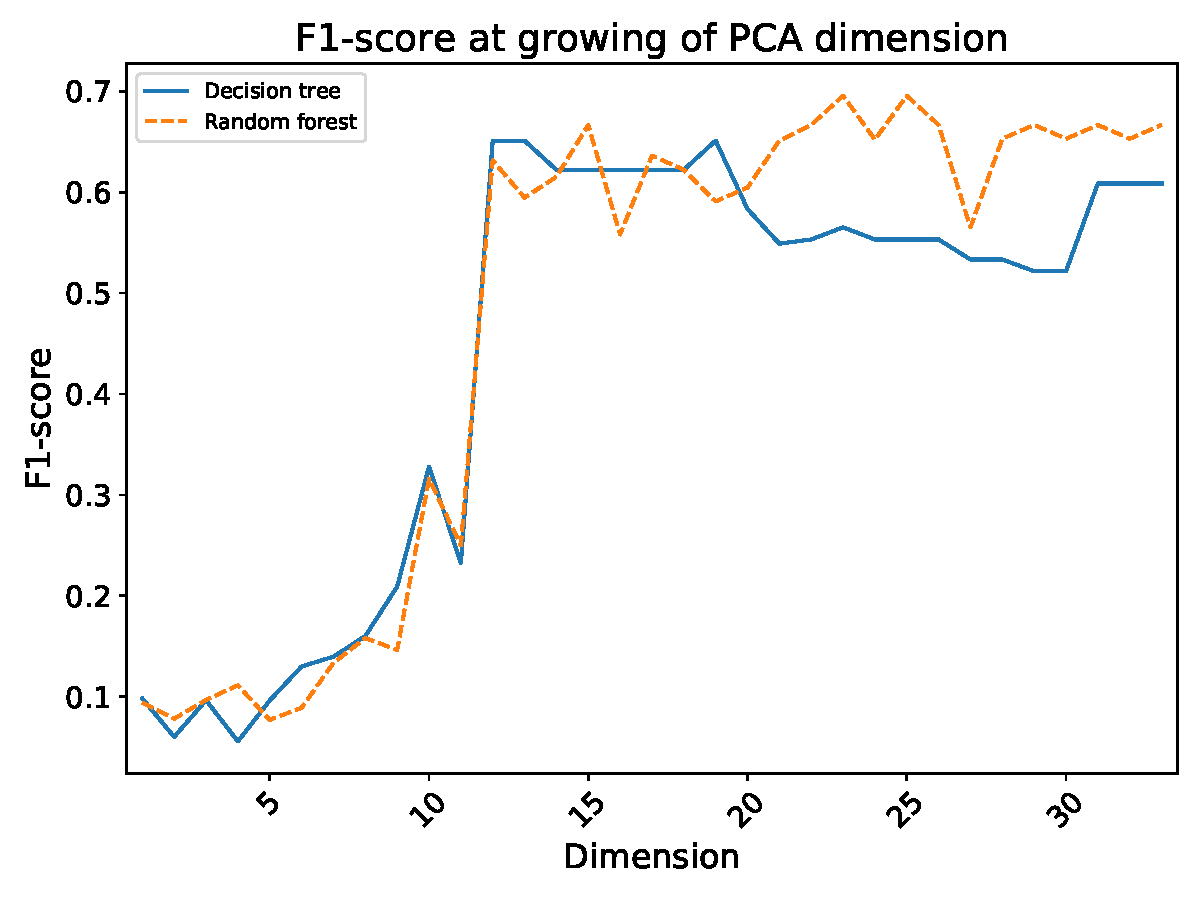
\includegraphics[width=0.9\linewidth]{images/pca-perf}
	\caption{}
	\label{fig:pca-perf}
\end{figure}


\begin{figure}
	\centering
	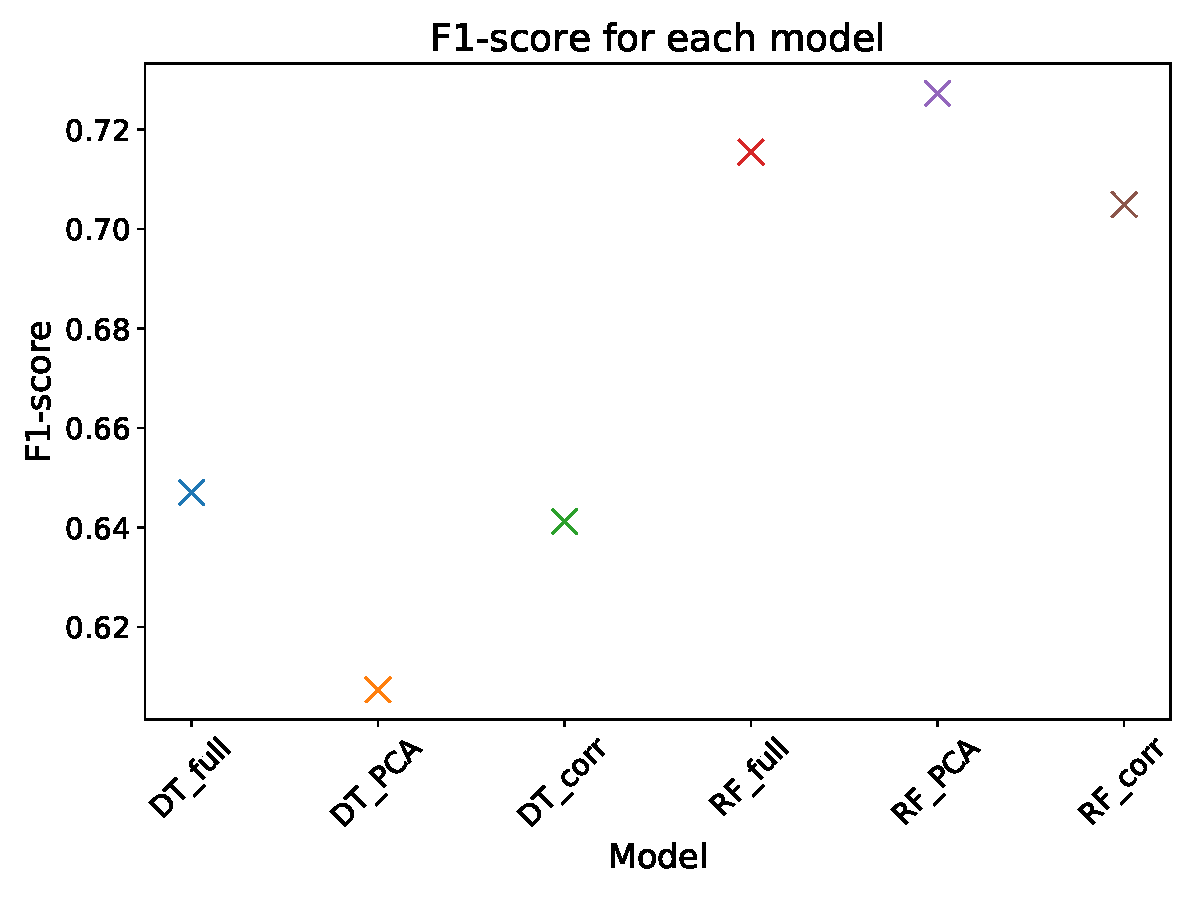
\includegraphics[width=0.8\linewidth]{images/fscore}
	\caption{}
	\label{fig:fscore}
\end{figure}

\todo[inline]{Citazione biblio è strana con o accentate grandi DP}